\chapter{TicTacToe, from a prompt to a checked game}\label{ch:walkthrough}

This chapter is a walk through a Claude Desktop session, in pictures: connect to LeanFM, ask for
TicTacToe, see its source, see what LeanFM generates from it, play it, check a small
implementation, and ask for a video. The video is \texttt{video/tictactoe/tictactoe-walkthrough.mp4},
and \texttt{make video-tictactoe} makes it again.

What is real and what is re-enacted: the chat frames are drawn, as a re-enactment, but every tool
answer in them is LeanFM's real one. Every screenshot of LeanFM's viewer is the real viewer, opened
by \texttt{make serve}'s standalone page on the protocol file. The game is the real TypeScript below,
played in a browser, and its log is checked by the real server.

\section{Connect}

One entry in Claude Desktop's configuration starts LeanFM's MCP relay, which talks to the server
\texttt{make serve} runs (Chapter~\ref{ch:start}). The first call to make is \texttt{introduction}:
what LeanFM is, the rule for writing requirements, and the calls to make next.

\begin{figure}[H]
\centering
\AccessibleFigure{A re-enacted Claude Desktop chat - the leanfm entry of the configuration the request Introduce LeanFM the introduction tool's answer and Claude's summary of it.}{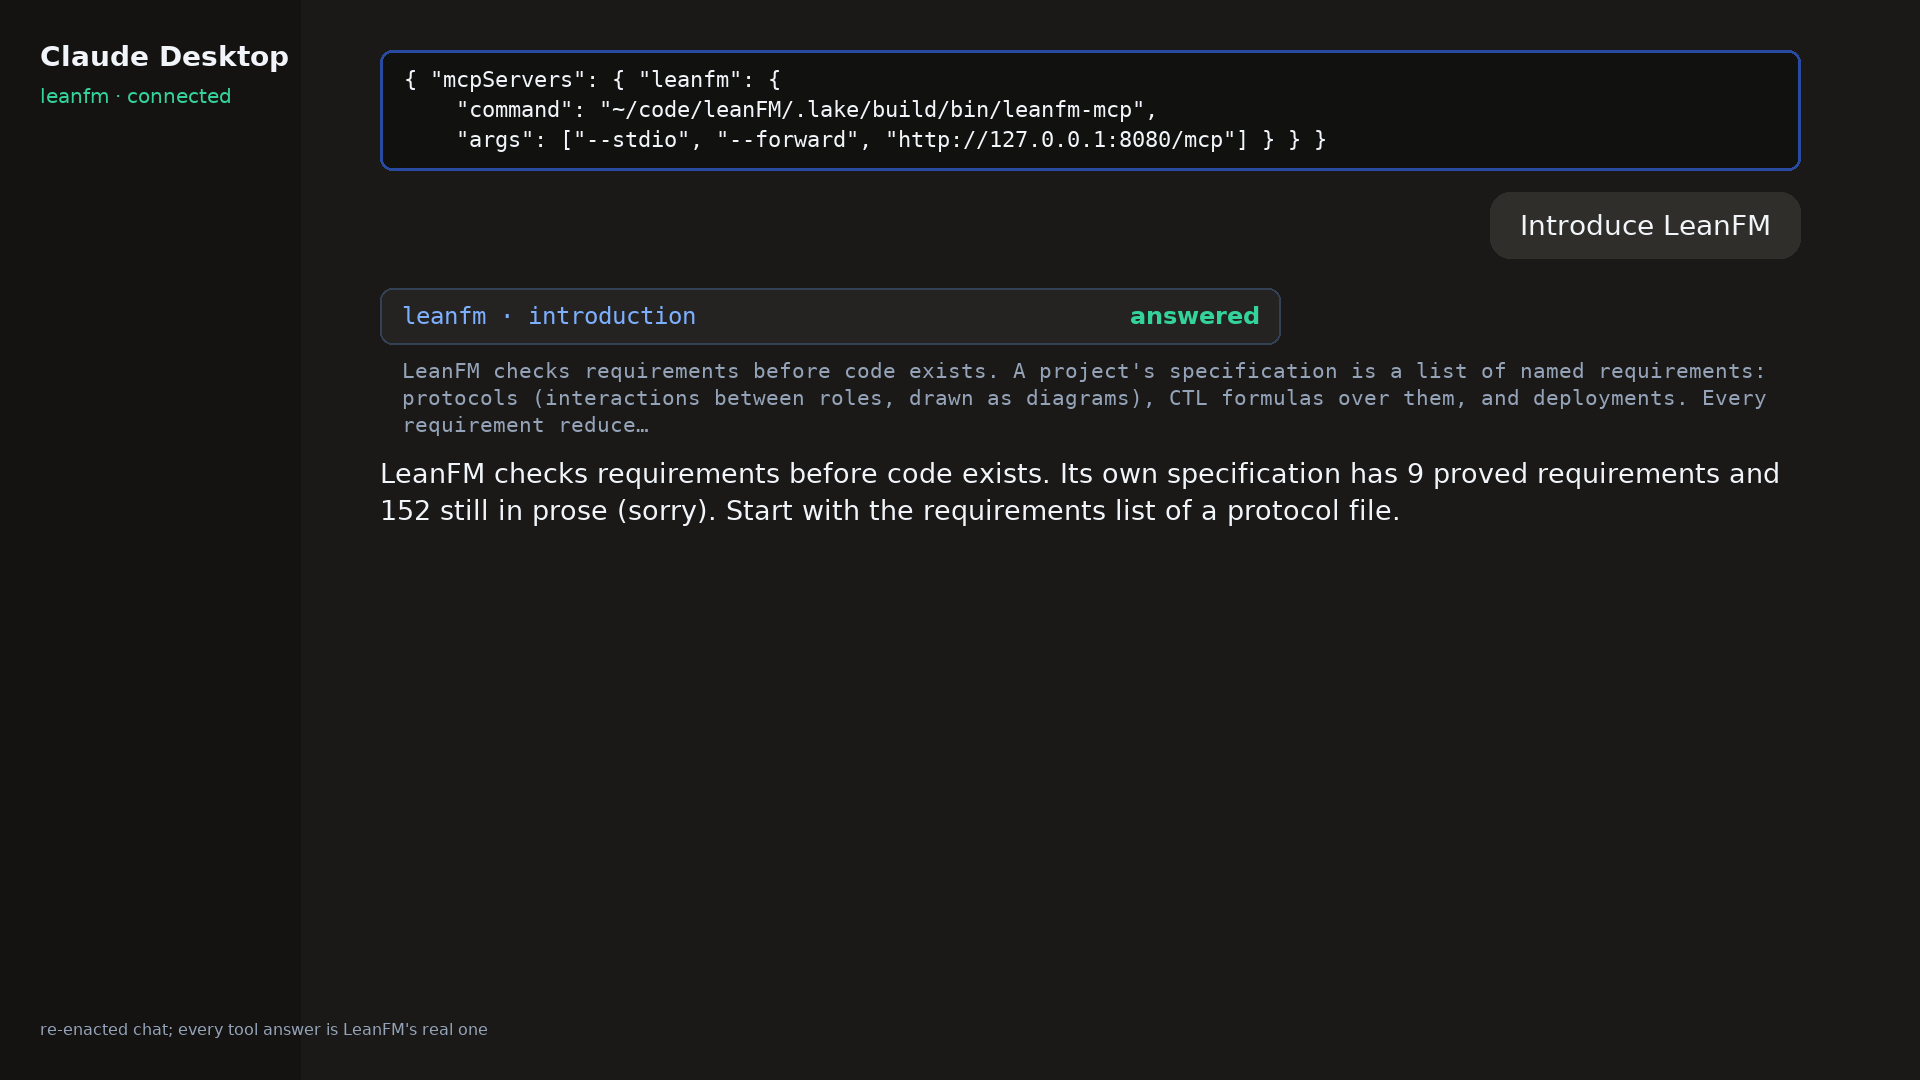
\includegraphics[width=\textwidth]{generated/walk-chat-connect.png}}
\caption{Connecting, and the introduction (re-enacted chat; the tool's answer is real).}
\end{figure}

\section{Ask for TicTacToe, and see its source}

Asked for a TicTacToe game, Claude writes it as a protocol with its requirements. This is the
source, written once; it is the file \texttt{examples/sessions/TicTacToe.leanfm}:

\lstinputlisting[firstline=6]{../examples/sessions/TicTacToe.leanfm}

\begin{figure}[H]
\centering
\AccessibleFigure{A re-enacted chat - the request Make a TicTacToe game Claude's reply with the protocol and session_check's answer.}{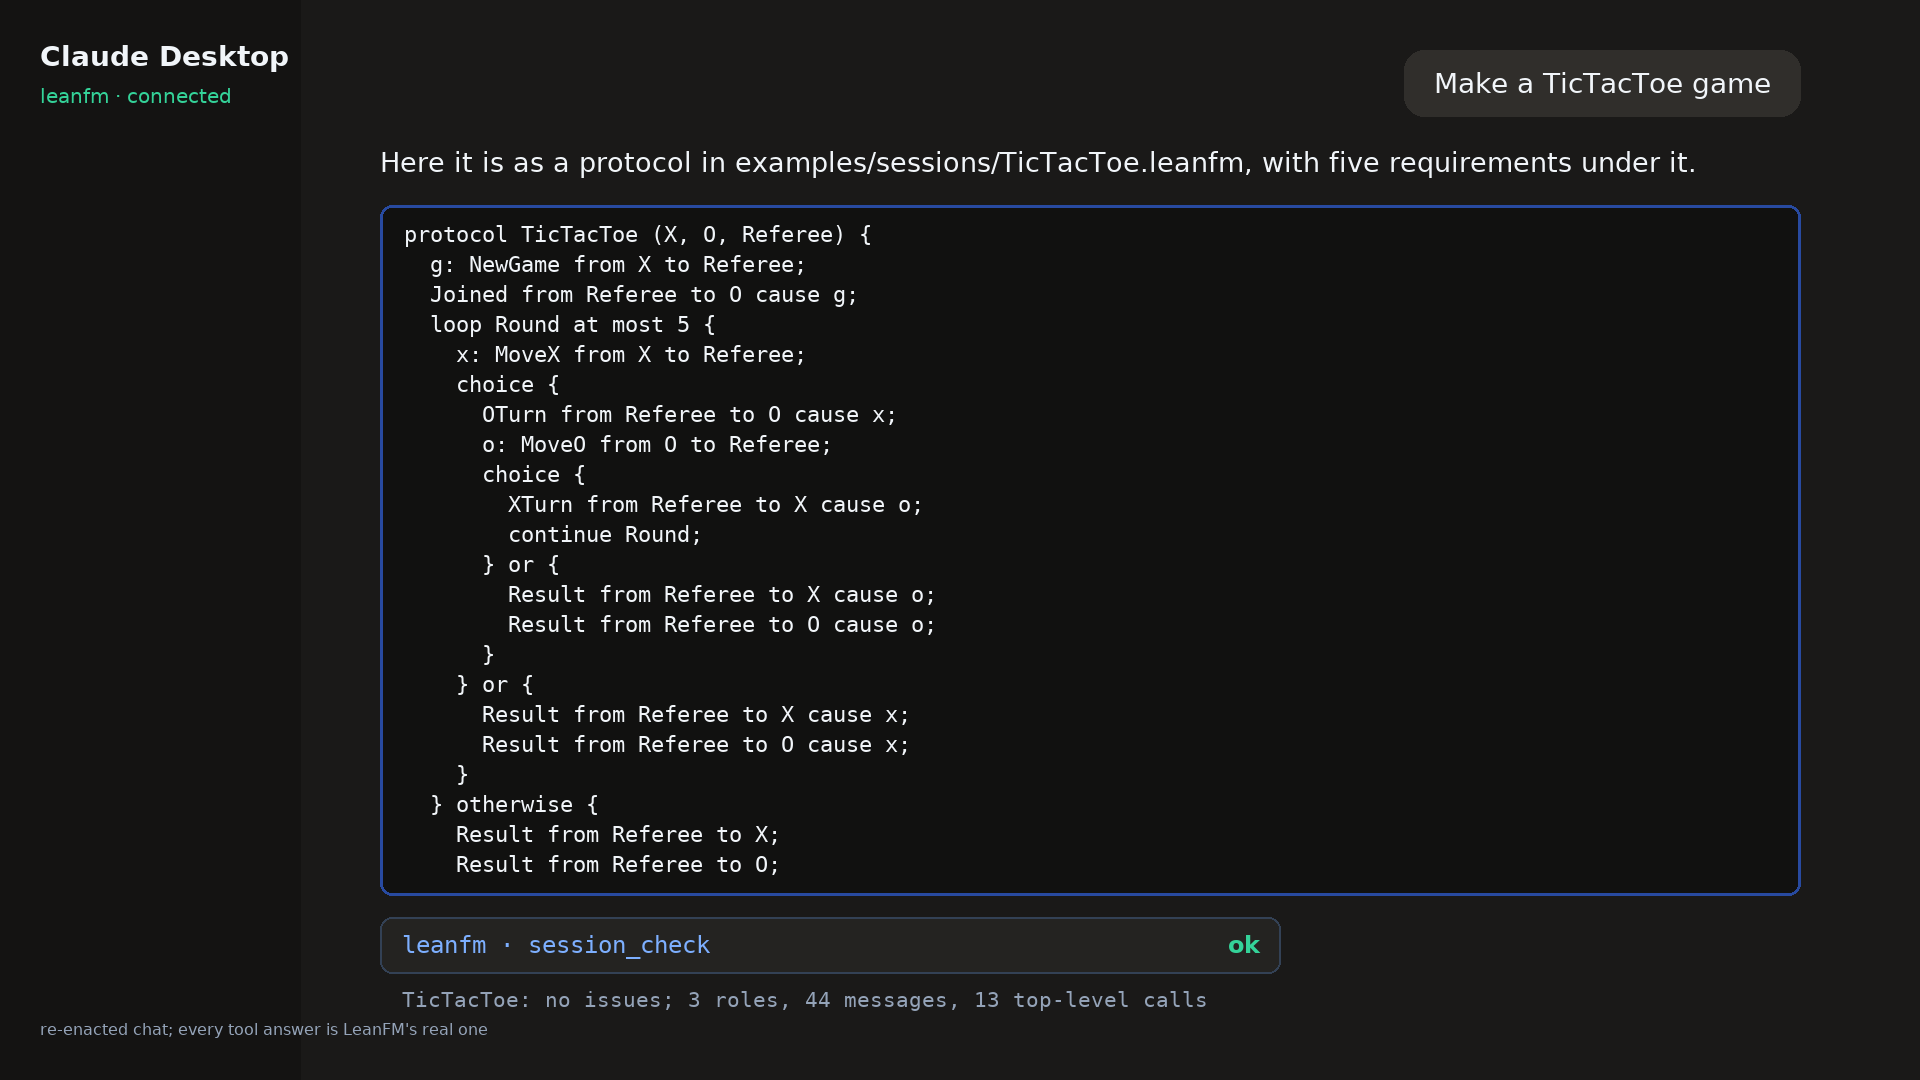
\includegraphics[width=\textwidth]{generated/walk-chat-prompt.png}}
\caption{The prompt and the protocol Claude wrote (re-enacted chat; session\_check's answer is real).}
\end{figure}

In the chat itself, LeanFM's viewer comes up inline, right under the tool call that drew it. Ask for
TicTacToe's requirements and the list appears in the conversation, ready to browse:

\begin{figure}[H]
\centering
\AccessibleFigure{A re-enacted chat - the request Show me TicTacToe's requirements the session_explore call and under it LeanFM's viewer inline with the requirements list of seven proved requirements.}{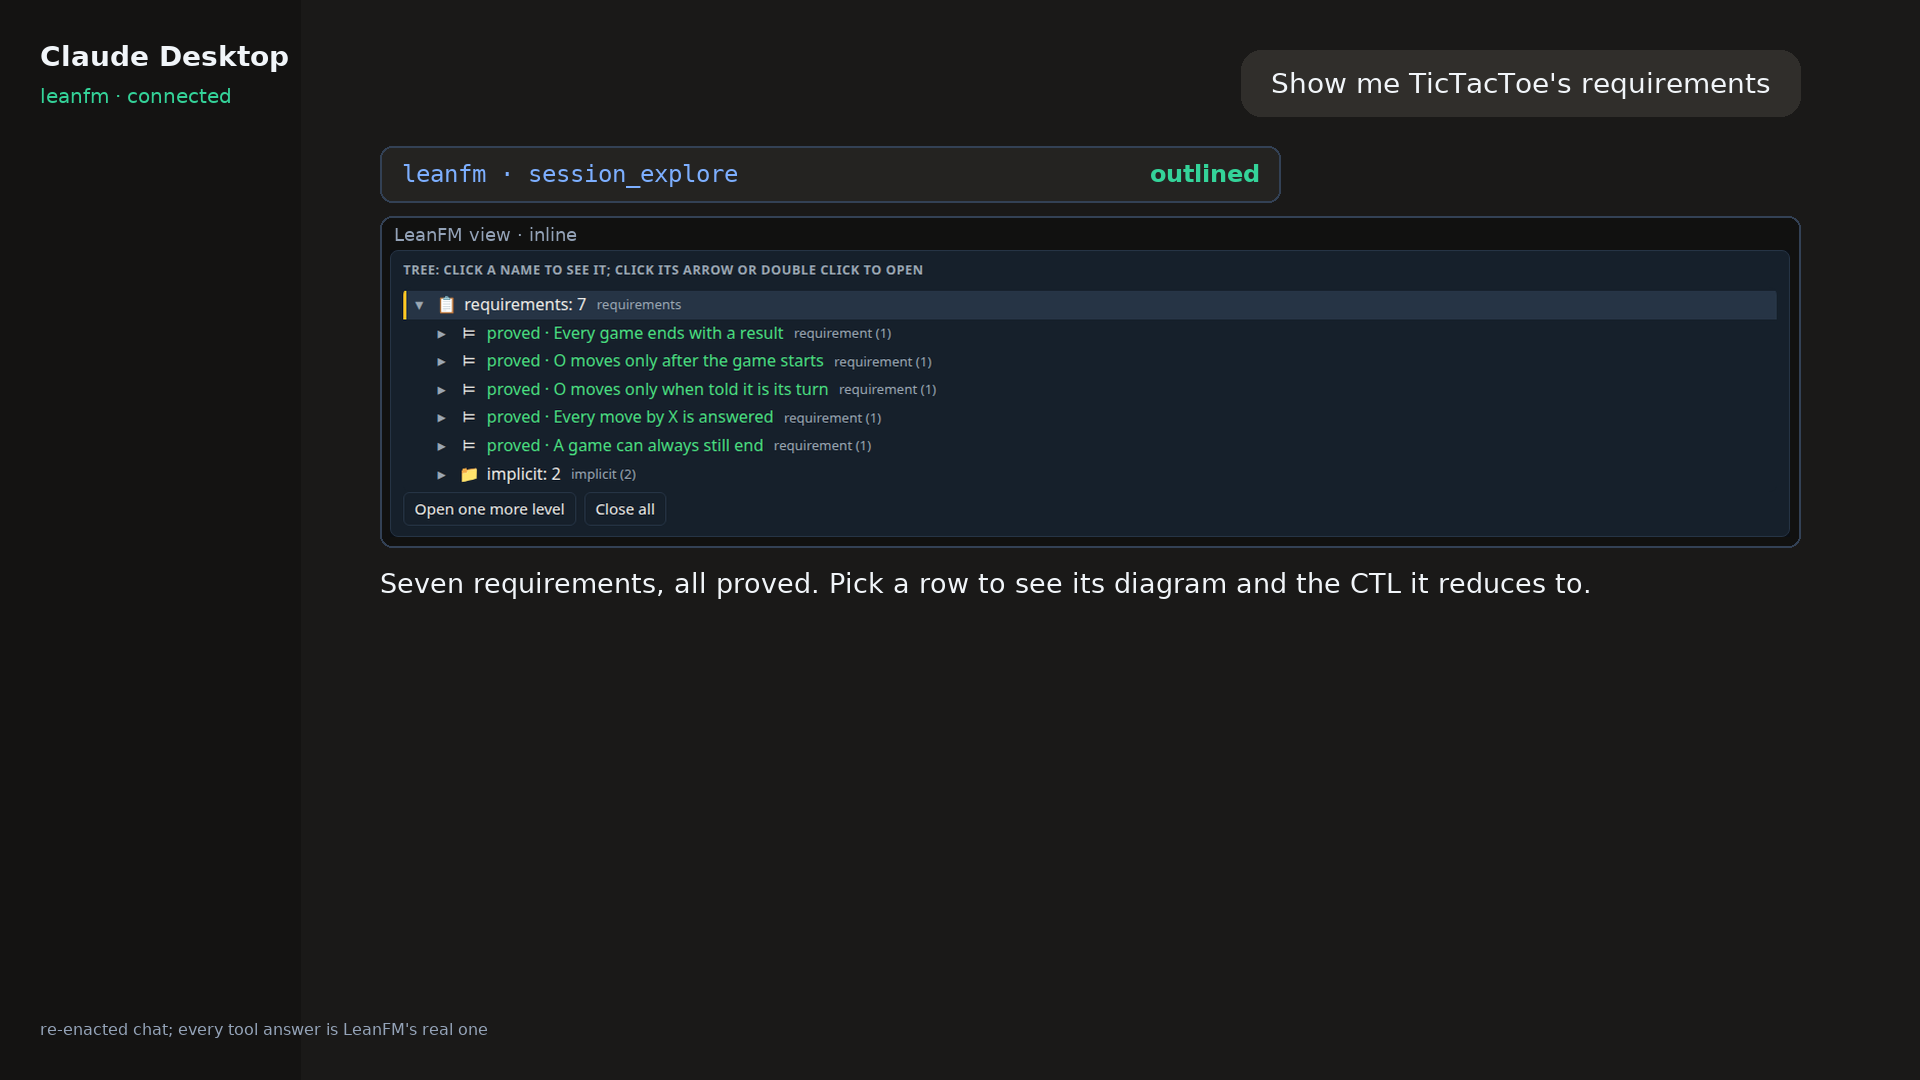
\includegraphics[width=\textwidth]{generated/walk-chat-inline.png}}
\caption{The viewer inline in the chat (re-enacted chat; the viewer inside it is a real screenshot).}
\end{figure}

\section{Here come the generated diagrams}

\noindent\fcolorbox{toolrule}{diagramblue}{\parbox{\dimexpr\linewidth-2\fboxsep-2\fboxrule\relax}{%
\color{foregroundink}\textbf{Everything in this section is generated by LeanFM from the protocol above.}
Nothing is drawn by hand: the requirements list, the interaction diagram and the simulated games
are LeanFM's answers, shown in LeanFM's viewer. Each has the double border of tool output.}}

\medskip
First the requirements list. Every row is a named requirement with its standing; the last two are
the requirements LeanFM demands of every protocol. Picking a row draws its protocol and opens the
CTL it reduces to.

\begin{figure}[H]
\centering
\AccessibleFigure{LeanFM's viewer showing TicTacToe's requirements list - requirements 7 five proved requirements by name and a folder implicit 2.}{\ToolShot{\textwidth}{walk-tree.png}}
\caption{TicTacToe's requirements, as \texttt{session\_explore} lists them.}
\end{figure}

Then the interaction diagram. The rounds are one loop, at most five, and each choice names the
role that decides.

\begin{figure}[H]
\centering
\AccessibleFigure{The sequence diagram of TicTacToe - NewGame from X to Referee Joined from Referee to O then a group Round at most 5 holding the loop Round - MoveX and a choice the Referee decides between OTurn then MoveO and a Result to each player; then a group otherwise after 5 with a Result to each player.}{\ToolShot{\textwidth}{walk-diagram.png}}
\caption{The interaction diagram, generated from the protocol.}
\end{figure}

And then play it. LeanFM's simulator generates games from the protocol alone and animates their
events. No implementation exists yet: these are runs the specification allows.

\begin{figure}[H]
\centering
\AccessibleFigure{The viewer's event stream for ten simulated TicTacToe sessions - a banner saying simulated not a real run the sessions the event log and the animated diagram.}{\ToolShot{\textwidth}{walk-animate.png}}
\caption{Simulated games: \texttt{session\_simulate}, not a real run.}
\end{figure}

\section{A small implementation, checked}

Then the code, kept small: TicTacToe in TypeScript, where the Referee writes every protocol message
to a log. O plays at random from a seed, so a game can be replayed.

\lstinputlisting[language={},basicstyle=\ttfamily\footnotesize]{examples/tictactoe.ts}

Played in a browser, with X taking the centre and the corners:

\begin{figure}[H]
\centering
\AccessibleFigure{The TicTacToe page - X has won along the diagonal and beside the board the Referee's log lists thirteen events from NewGame to the two Results.}{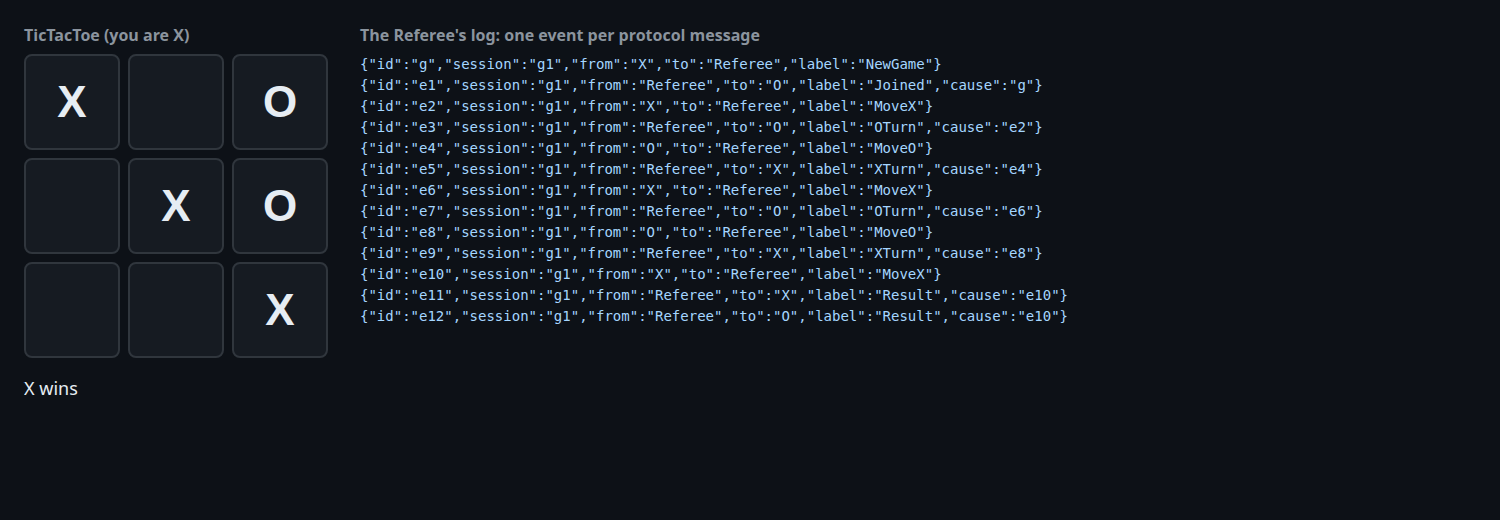
\includegraphics[width=\textwidth]{generated/walk-game.png}}
\caption{The implementation, played, with the Referee's log beside the board.}
\end{figure}

LeanFM checks that log against the protocol:

\ToolOutput{generated/walk-conform.tex}

\section{Ask for a video}

Last, ask for a video of the whole walkthrough. The same capture and a local narration make it from
the specification, so a video can be the prompt for the code, made before any code exists.

\begin{figure}[H]
\centering
\AccessibleFigure{A re-enacted chat - the request Make a video of this walkthrough Claude running make video-tictactoe and the line saying the video was written.}{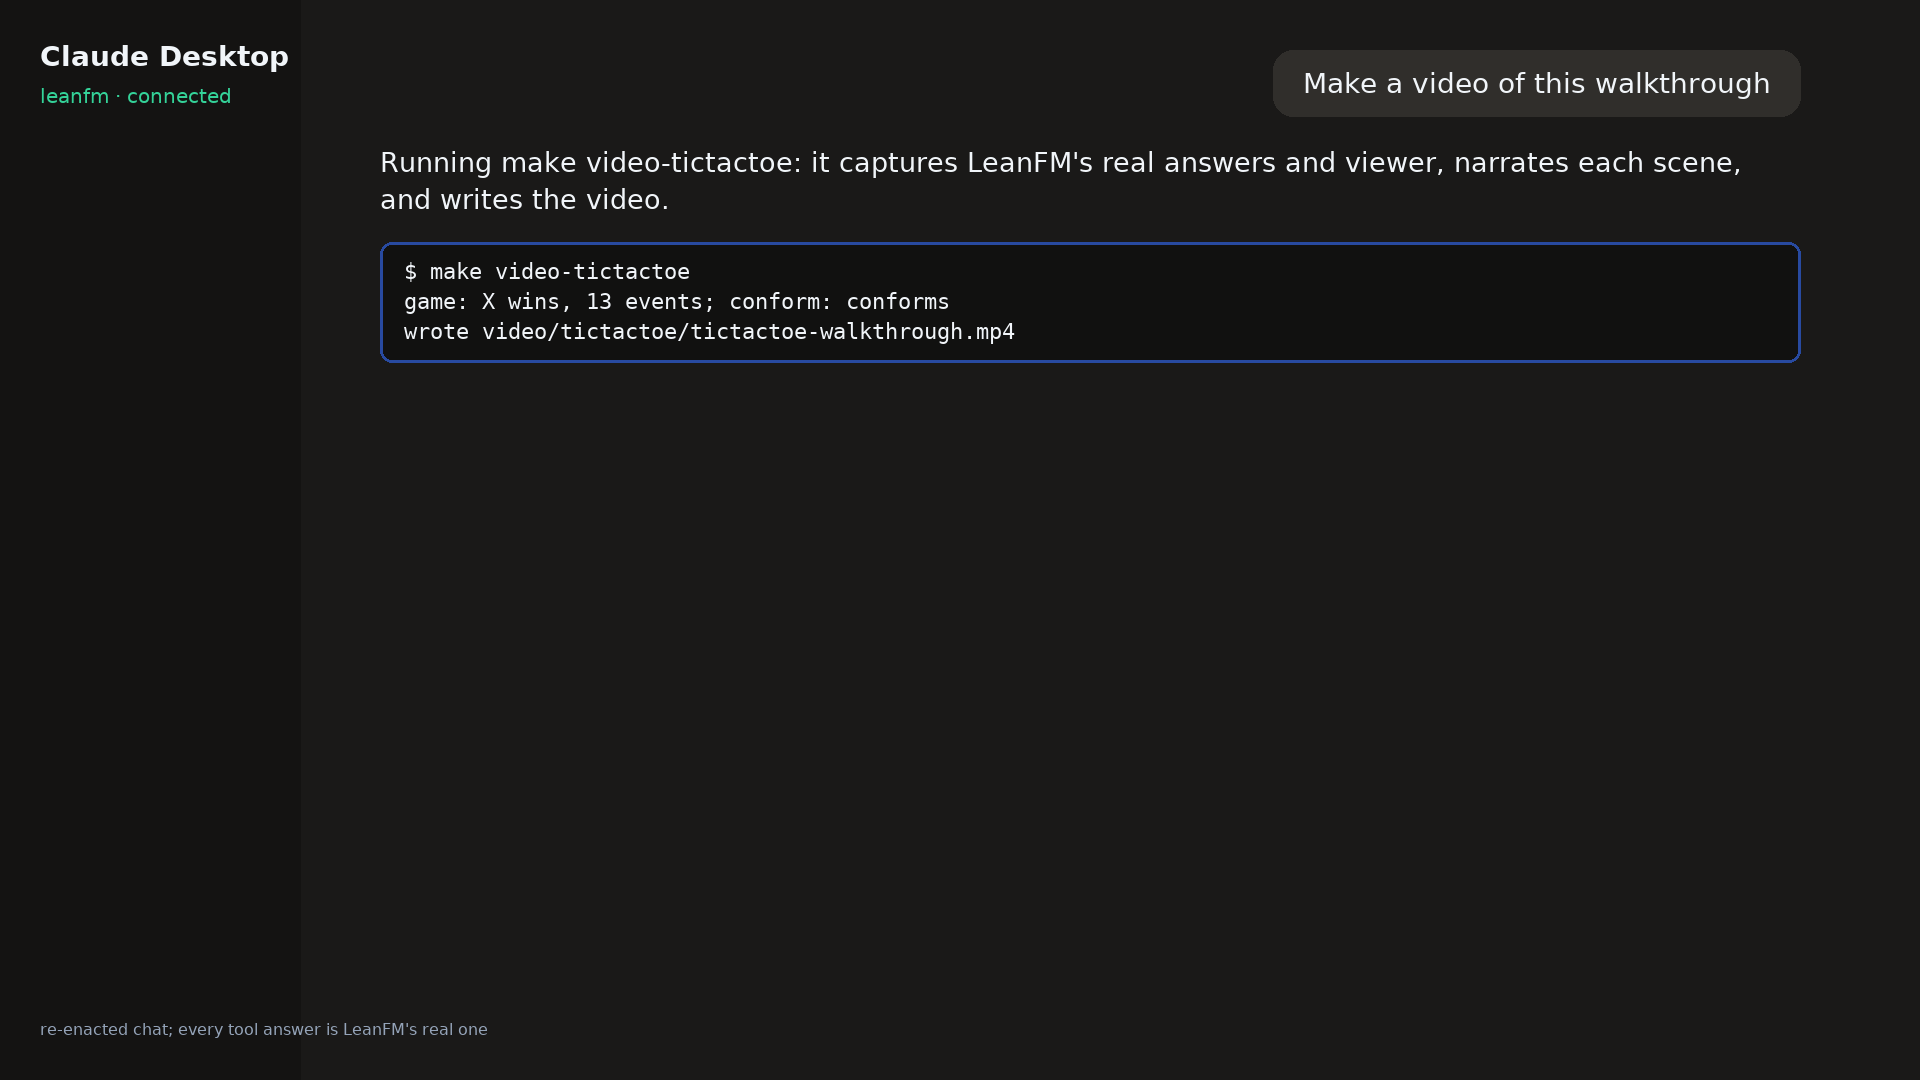
\includegraphics[width=\textwidth]{generated/walk-chat-video.png}}
\caption{Asking for the video (re-enacted chat; the command's output is real).}
\end{figure}
